\documentclass[a4paper]{article}
\usepackage[top=10mm,bottom=10mm,inner=10mm,outer=10mm]{geometry}
\usepackage{tikz}
\begin{document} 
\pagestyle{empty}
\centering
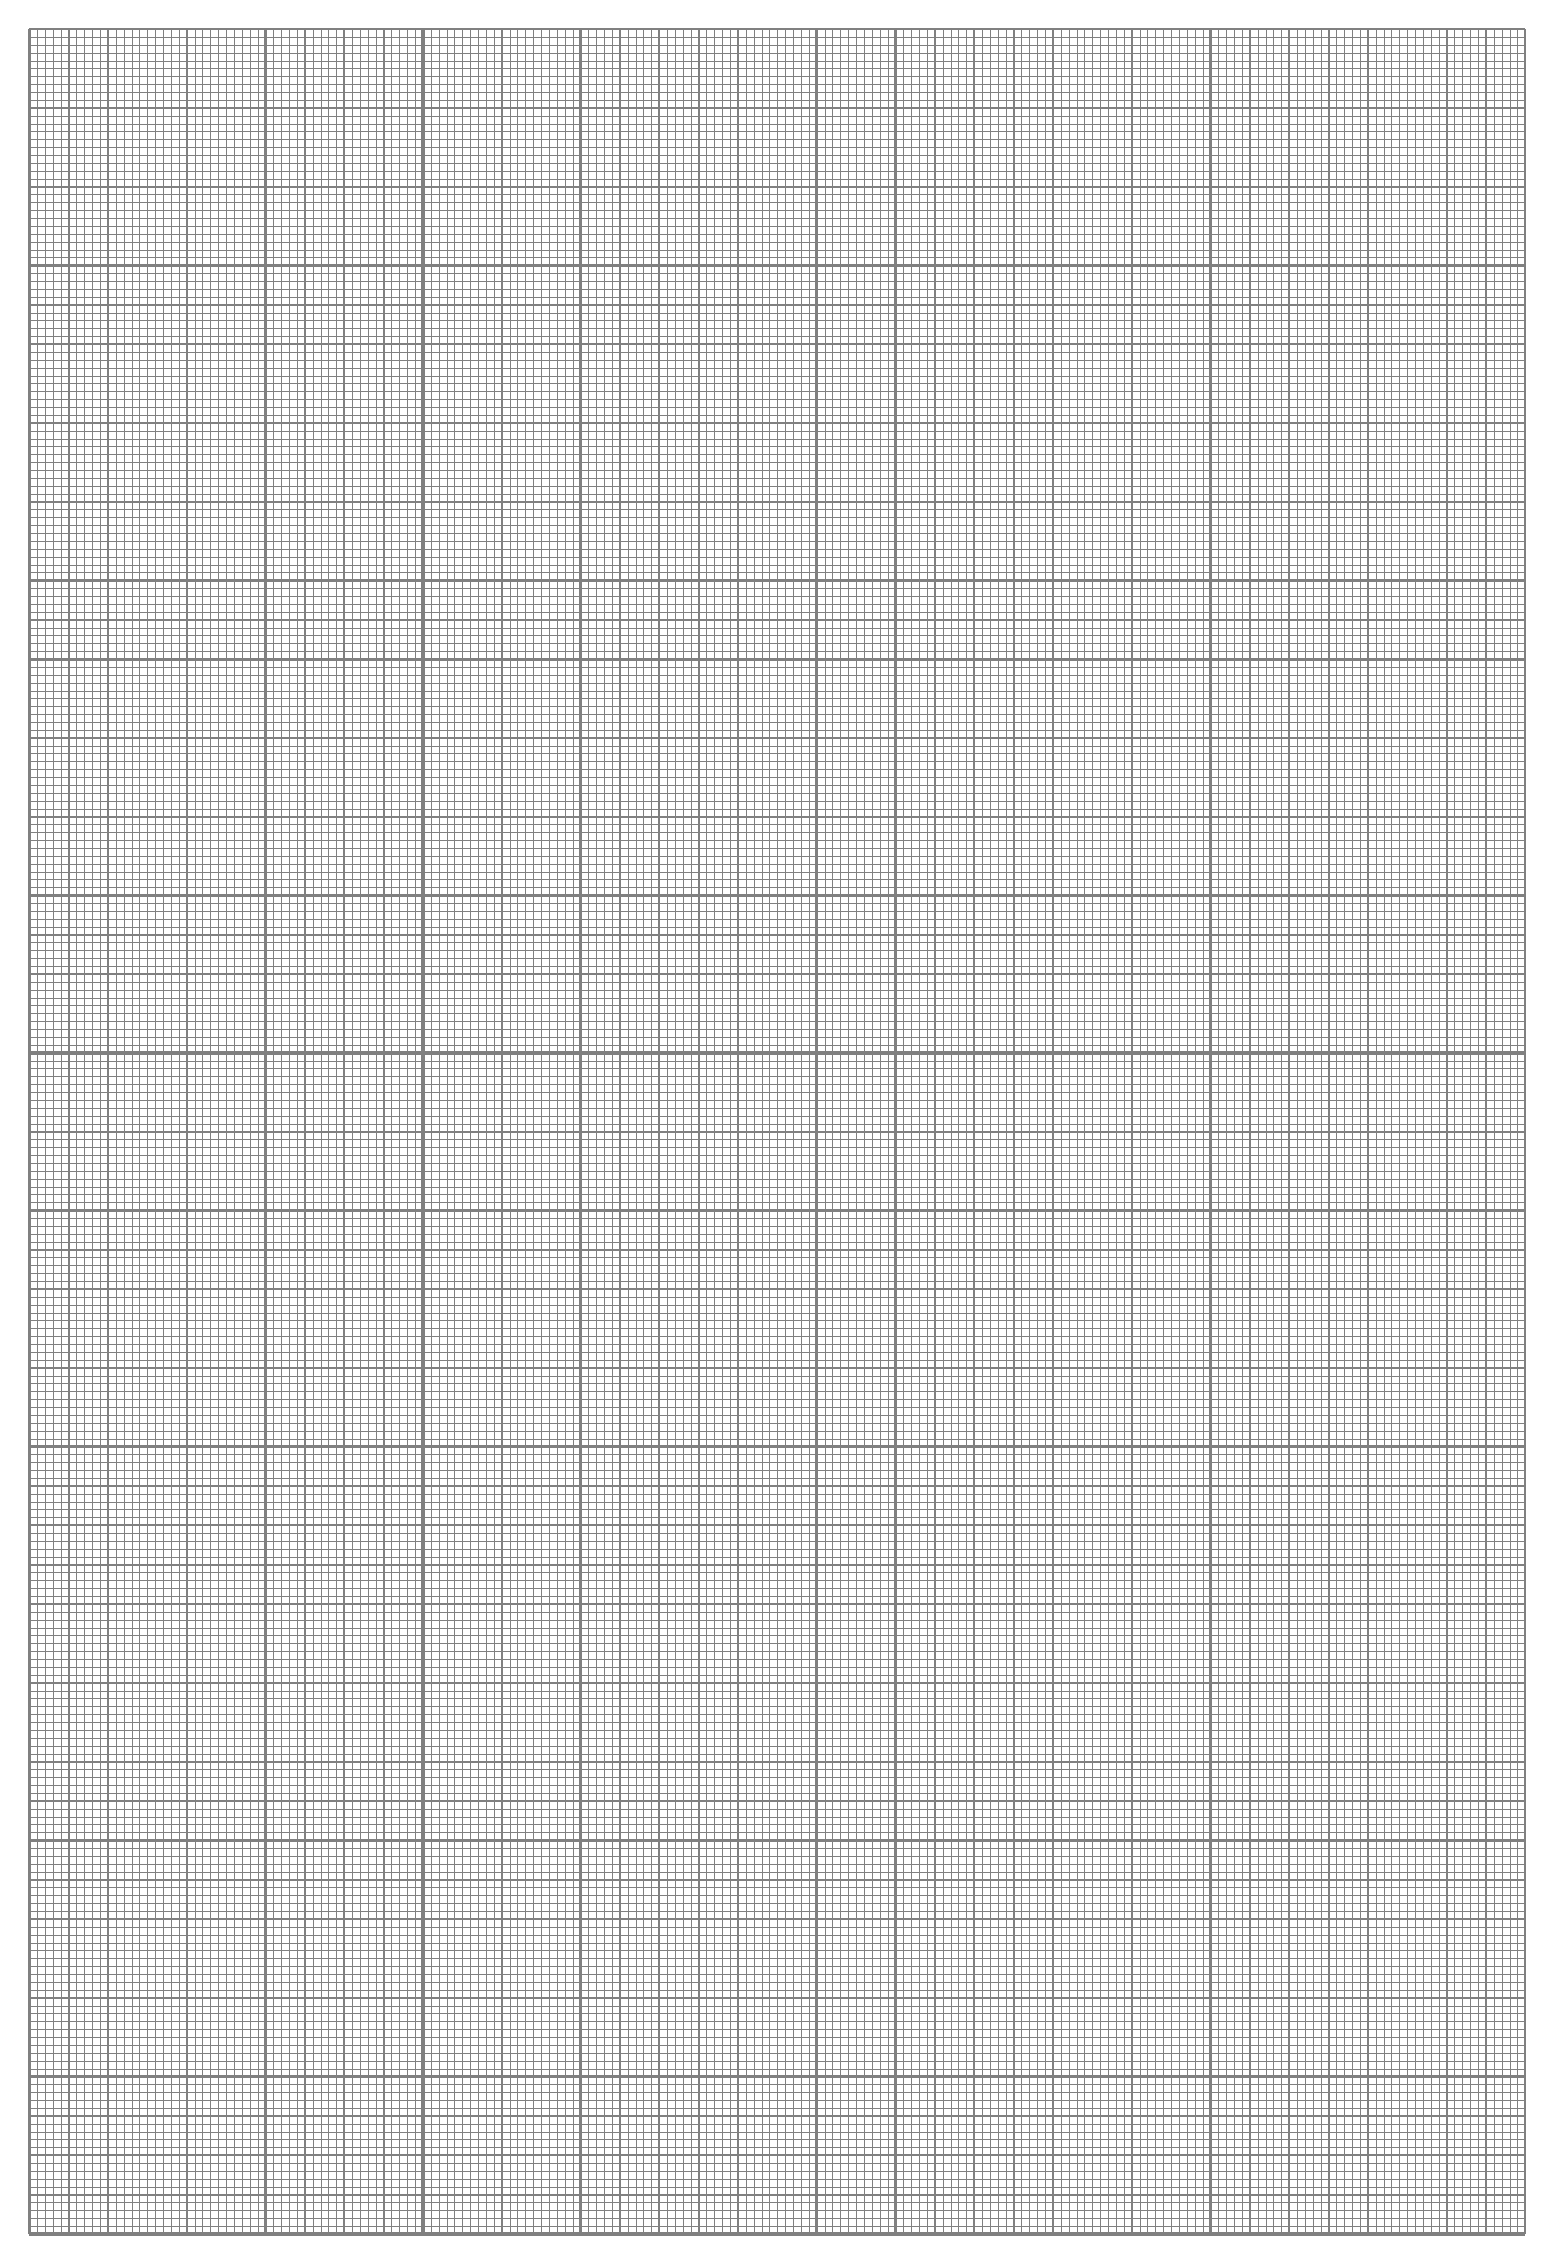
\begin{tikzpicture}
	% Dimensions du repere
	\def\xmin{0} \def\xmax{19} \def\ymin{0} \def\ymax{28}
	% Grilles
	\draw [step=0.1cm,gray,ultra thin]  (\xmin,\ymin) grid (\xmax,\ymax);
	\draw [step=0.5cm,gray, thin] (\xmin,\ymin) grid (\xmax,\ymax);
	\draw [step=1cm,gray, thick] (\xmin,\ymin) grid (\xmax,\ymax);
	\draw [step=5cm,gray,very thick] (\xmin,\ymin) grid (\xmax,\ymax);

	%\draw [step=0.25cm,gray,very thin] (\xmin,\ymin) grid (\xmax,\ymax);
	%\draw [step=1cm,gray,thin] (\xmin,\ymin) grid (\xmax,\ymax);
	%\draw [step=5cm,thick,color=black]  (\xmin,\ymin) grid (\xmax,\ymax); 	
\end{tikzpicture}
\end{document} 